\section{Example of CFPQ With Combinators}

In this section we demonstrate main features of combinators in the context of context-free path querying and integration with general-purpose programming languages.
To do it we first introduce a simple graph analysis problem and then show how to solve it by using parser combinators.
In our wirk we use Merrkst.Graph combinators library.

\underline{\textbf{Problem statement.}}
Suppose we have an RDF graph and whatn to analize hierarchical dependencies over different types of relations.
Our goal is for fhe given object to find all objects which lies on the same lavel of hierarchy.
Namely, for the given set of relations $r = \{R_0 \ldots R_i\}$ and for the given vertex $v$ we want to find all vertices reachable form $v$ by paths which specified by the following context free grammar in EBNF: 
%\begin{align*} 
 %\textit{qSameGen} \to & {R_0}^{-1} R_0 \mid \ldots {R_i}^{-1} R_i  \mid \\
 %                      & {R_0}^{-1} \textit{qSameGen } R_0 \mid \ldots \mid {R_i}^{-1} \textit{qSameGen } R_i.
 $\textit{qSameGen} \to {R_0}^{-1} \textit{qSameGen? } R_0 \mid \ldots \mid {R_i}^{-1} \textit{qSameGen? } R_i.$
 %\end{align*}
Additionally we want to calculate lenght of these paths.

%\subsection{Simple Solution}

The first step is to specify paths constraint. 
For example, we fix relation to be \verb|skos__narrowerTransitive|.
Then constraint may be specified in terms of combinators as follows:

\begin{lstlisting}
val rName = "skos__narrowerTransitive"
def qSameGen () =
    syn(inE((_: Entity).label() == rName) ~ qSameGen().? ~
        outE((_: Entity).label() == rName))
\end{lstlisting}

Here we use \verb|inE| and \verb|outE| to specify incoming nad outgoing edges with respective label, \verb|~| to concatenate subqueryes, and \verb|.?| to specify zero or one repitition of subquery.

This query specifies exactly path we want, but still not a solution.
First of all, we can not specify start vertex and can not extract final vertices.
Also, this query is for one specified relation.
To investigate hierarchy over a set of relations we need to rewrite it.

\underline{\textbf{Compositionality.}}
First step is a generalization of the query to simplfy handling of different types of relations.
To do it we introduce a helper function \verb|reduceChoice| which takes a list of subqueryes and combine them by using alternation operation.

\begin{lstlisting}
def reduceChoice(qs: List[_]) =
  qs match {
     case x :: Nil => x
     case x :: y :: qs => syn(qs.foldLeft(x | y)(_ | _))
  }
\end{lstlisting}

After that we use this function in new version of \verb|sameGen| to combine subqueryes for different types of braces.
To make it possible to use differetn types of braces without query rewriting we pass barces as a parameter.

\begin{lstlisting}
def sameGen(brs: List[(_,_)]) =
    reduceChoice( brs.map {
      case (lbr, rbr) => syn(lbr ~ sameGen(brs).? ~ rbr)
      })
\end{lstlisting}

Now we are ready to provide ability to specify start vertex and collect information of final vertices.
First of all, we provide a filter to select only vertices with \verb|uri| property.

\begin{lstlisting}
val uriV = syn(V((_: Entity).hasProperty("uri")) ^^)
\end{lstlisting}

After thet we create a function which takes two parameters, start vertex and a path query, and create a new query to find all vertices with \verb|uri| property which are reachcbl from the specified strat vertex by specified path.
Finally we collect values of \verb|uri| for all reachable vertices.
To do it we specify user-defined action {\small \verb|{case _ ~ _ ~ (v: Entity) => v.getProperty[String]("uri")}|} which captures result of query (it is a triple-sequence of subqueryes results) and gets the \verb|uri| property form result of last subquery.

\begin{lstlisting}
def queryFromV (startV, query) =
  syn(startV ~ query ~ uriV &
      {case _ ~ _ ~ (v: Entity) =>
            v.getProperty[String]("uri")})
\end{lstlisting}


\underline{\textbf{User-defined actions.}}
Final step is to extend the query with calculation of lengths of all paths which satisfie conditions.
To do it we equip \verb|sameGen| with additional user-defined actions.

\begin{lstlisting}
def sameGen(brs: List[(_,_)]) =
    reduceChoice(
      brs.map {
        case (lbr, rbr) =>
          syn((lbr ~ (sameGen(brs).?) ~ rbr) & {
            case _~Nil~_ => 2
            case _~((x:Int)::Nil)~_ =>  x + 2
          })
      })
\end{lstlisting}

The \verb|queryFromV| now handles not only theard element, but also the second one in order to get access to accamulated lenghts.

\begin{lstlisting}
def queryFromV(startV, query) =
    syn(startV ~ query ~ uriV &
      {case _ ~ (len:Int) ~ (v:Entity) =>
        (len, v.getProperty[String]("uri"))})
\end{lstlisting}

\begin{lstlisting}
def makeBrs (brs:List[_]) =
    brs.map(name =>
       (syn(inE((_: Entity).label() == name) ^^),
        syn(outE((_: Entity).label() == name) ^^)))
    .toList
    
def runExample (brs: List[_], startVId, graph) =
    val startV = V(getIdFromNode(_: Entity) == startVId
    executeQuery(queryFromV( syn(startV)^^),
                               sameGen(makeBrs(brs))),
                   graph).toList

runExample(RdfConstants.RDFS__SUB_CLASS_OF :: Nil, 1, graph)
\end{lstlisting}



\underline{\textbf{Type safety.}}
If subqueryes are composed incorrectly, then

In example showed in figure~\ref{fig:types}, elements of pair wich represents query result are used incorrectly: we want to find total length of all paths but sum final vertices' identifiers instead of lenghths.
As a result, compiler statically detect a error because integer expected instead of string.

\begin{figure}[ht]
   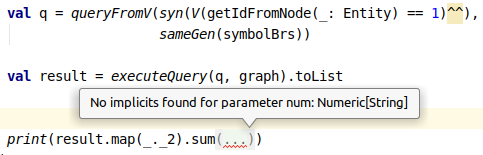
\includegraphics[width=0.48\textwidth]{pictures/image.png}
   \caption{!!!}
   \label{fig:types}
\end{figure}

\underline{\textbf{IDE Support.}}
Since you can use IDE for development, you get all features for qury development, such as syntah highkighting, code navigation, autocompletion, without any additional effor.
An example of autocompletion suggestions for vertex is presented in figure~\ref{fig:autocompletion}.

\begin{figure}[ht]
    \centering
    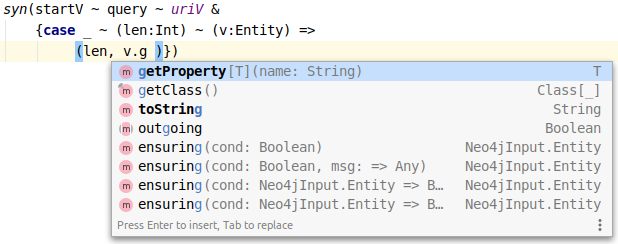
\includegraphics[width=0.48\textwidth]{pictures/image1.png}
    \caption{!!!!}
    \label{fig:autocompletion}
\end{figure}
